\documentclass[24pt,pdf,hyperref={unicode}]{beamer}
\usepackage[utf8]{inputenc}
\usepackage[russian]{babel}
\usepackage{aiml}

\begin{document}

\section{Рождение теории (1936-1956)}

\begin{frame}
\bio{Turing}{Алан Тьюринг}{

On computable numbers, with an application to the Entscheidungsproblem (1936)

Computing machinery and intelligence (1950)
}
\end{frame}

\begin{frame}
\citate{
Машину, каждое перемещение которой ... полностью определено ее конфигурацией, мы будем называть автоматической машиной (or $a$-machine).

Однако для некоторых целей мы можем использовать машины ($c$-машины), чье поведение только частично определено их конфигурацией. 
... Когда такая машина достигает неоднозначной конфигурации, она останавливается до тех пор, пока внешний оператор не выберет
какой-либо вариант продолжения. В этой статье я рассматриваю лишь автоматические машины, и потому опускаю префикс $a$.

}{Alan Turing}{On computable numbers, with an application to the Entscheidungsproblem}
\end{frame}

 

\begin{frame}
\citate
{
Поведение компьютера в каждый момент времени определено символами, который он наблюдает, и его ``состоянием сознания''. 
Мы можем считать, что количество таких символов ограничено в каждый момент времени сверху границей $B$. Если компьютеру нужно рассмотреть 
больше символов, необходимо использовать последовательные наблюдения. Мы также можем считать, что количество его состояний сознания также конечно.
}{Alan Turing}{On computable numbers, with an application to the Entscheidungsproblem}
\end{frame}

\begin{frame}
\citate
{
The behaviour of the computer at any moment is determined by the symbols which \alert<2->{he} is observing, and \alert<2->{his "state of mind"} at that moment. We may suppose that there is a bound $B$ to the number of symbols or squares which the computer can observe at one moment. If \alert<2->{he wishes} to observe more, he must use successive observations. We will also suppose that the number of \alert<2->{states of mind} which need be taken into account is finite.
}{Alan Turing}{On computable numbers, with an application to the Entscheidungsproblem}
\end{frame}

\begin{frame}
\citate
{
[Рассмотрим] игру, которую мы будем называть ``игрой в имитацию''. В нее играют мужчина (A), женщина (B), и жюри (C). Жюри располагается в отдельной от остальных комнате. Цель жюри состоит в том, чтобы определить, кто из игроков мужчина, а кто -- женщина, [цель игроков -- запутать жюри]. Жюри знает игроков по меткам X и Y. Далее жюри задает вопросы, например:\\[0.2cm]

C: X, какая у вас длина волос? \\[0.2cm]

Предположим, что X -- это мужчина, и X отвечает:\\[0.2cm]

``У меня стрижка под фокстрот, а самые длинные пряди около 20 сантиметров''
}{Alan Turing}{Computing machinery and intelligence}
\end{frame}

\begin{frame}
\begin{center}
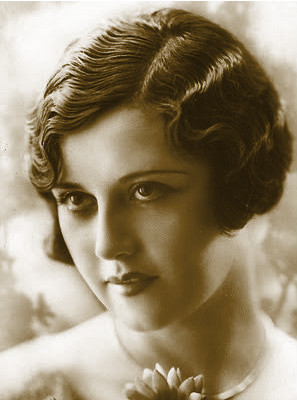
\includegraphics[width=0.4\textwidth]{Portraits/Shingled.jpg}
\end{center}
\end{frame}


\begin{frame}

\citate
{
Зададимся теперь вопросом, ``Что бы случилось, если бы машина заняла место A в этой игре?'' Может быть, жюри бы ошиблось? Этим вопросом мы заменим наш начальный вопрос, ``Может ли машина мыслить?''.
}{Alan Turing}{Computing machinery and intelligence}

\end{frame}

\begin{frame}
\doublebio
{McCulloch}{Warren McCulloch}
{Pitts}{Walter Pitts}
{A Logical Calculus of the Ideas Immanent in Nervous Activity (1943)}
\end{frame}

\begin{frame}
\bio{Barricelli}{Nils Aal Bariccelli}{Esempi Numerici di processi di evoluzione (1954)}
\end{frame}

\begin{frame}
\citate
{
Мы предлагаем двухмесячный исследовательский семинар в составе десяти человек для исследования искусственного интеллекта в течение лета 1956 года в Дортмундском колледже Гановера, Нью-Хэмпшир. Отправной точкой исследования является убеждение в том, что все аспекты обучения, и других проявлений интеллекта, могут быть настолько точно описаны, что машина может запрограммирована на их выполнение. Будет сделана попытка выяснить, как машины могут использовать язык, делать абстракции, решать различные виды задач, которые пока решает лишь человек, и самообучаться. Мы полагаем, что возможно существенное продвижение в этом вопросе, если тщательно отобранная группа ученых будет совместно работать над ним в течение лета.
}{McCarthy et al.}{Proposal for the project}
\end{frame}

\section{Золотой век (1957-1972)}

\begin{frame}
\begin{center}
 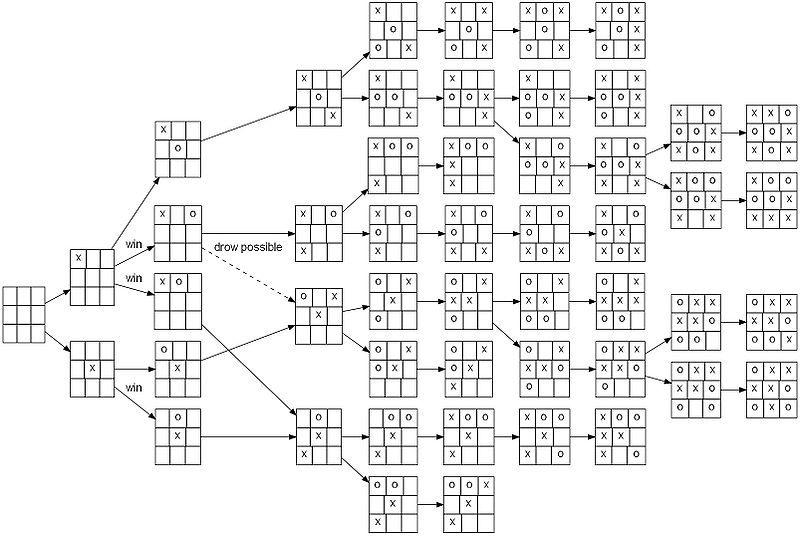
\includegraphics[width=\textwidth]{tictactoe.jpg}
\end{center}
\end{frame}


\begin{frame}
\bio{Robinson}{John Alan Robinson}{A Machine-Oriented Logic Based on the Resolution Principle (1965)}
\end{frame}


\begin{frame}
\bio{Rosenblatt}{Frank Rosenblatt}{Principles of neurodynamics: Perceptrons and the theory of brain mechanisms (1962)}
\end{frame}

\begin{frame}
\bio{Holland}{John Henry Holland}{Adaptation in Natural and Artificial Systems (1975)}
\end{frame}


\begin{frame}
\bio{Unimate}{UNIMATE}{Первый промышленный робот (1961)}
\end{frame}


\begin{frame}
\citate
{
В течение трех-восьми лет интеллект машины сравняется с общим интеллектом среднего человека. Я имею в виду, что машина сможет читать Шекспира, обслуживать автомобиль, заниматься политикой, рассказывать анекдоты и спорить. В этот же момент, машина начнет самообучаться с невероятной скоростью. В течение нескольких месяцев она достигнет уровня гения, а дальше ее возможности станут невообразимыми. 
}{Marvin Minsky}{Quoted by Life, 1970}
\end{frame}

\section{Первая зима (1973-1980)}

\begin{frame}


\doublebio
{Minsky}{Marvin Lee Minsky}
{Papert}{Seymour Papert}
{Perceptrons: an introduction to computational geometry (1969)}

\end{frame}


\begin{frame}
\bio{Lighthill}{Michael James Lighthill}{Artificial Intelligence: A General Survey (1973)}
\end{frame}

\begin{frame}
\citate
{\small
Иногда говорят, что мотивацией мужчин для работы ... в ``чистой науке'' является компенсация невозможности рождения детей. Если это правда, то Building Robots -- это идеальная компенсация! ... большая часть роботов построена так, что функционирует в соответствии с представлениями мужчин о мире ребенка: роботы играют в игры, разгадывают головоломки, описывают словами картинки (вроде ``медведя на коврике с мячом''). Но богатая эмоциональная составляющая детства полностью отсутствует. На это обычно отвечают, что робототехника -- молодая наука, а потому роботы способны имитировать лишь детские действия. Однако, автор пришел к ... мнению, что отношения между роботами и их строителями напоминают псевдо-детско-родительские.}{Charles Lighthill}{Artificial Intelligence: A General Survey}
\end{frame}

\begin{frame}
 \bio{Moravec}{Hans Moravec}{Mind Children: the future of robot and human intelligence (1988)}
\end{frame}

\begin{frame}
\citate
{\small
Сравнительно легко добиться от компьютера прохождения тестов на интеллект или игры в шашки на уровне взрослого человека; и тяжело или не возможно -- дать ему уровень годовалого ребенка, когда речь заходит о восприятии или движениях.}{Hans Moravec}{Mind Children: the future of robot and human intelligence}
\end{frame}


\begin{frame}
 \bio{Searl}{John Searl}{Minds, Brains and Programs (1980)}
\end{frame}

\section{Бум (1980-1986) }

\section{Вторая зима (1987-1993)}

\section{Новое время (1993-н.в.)}



\end{document}
